\documentclass{homework}

\usepackage{tcolorbox}
\usepackage{etoolbox}
\usepackage{svg}
\usepackage{algorithm}
\usepackage{algpseudocode}
\usepackage{caption}
\usepackage[newfloat]{minted}
\usepackage{pgfplots}
\usepackage{tabularx}
\pgfplotsset{width=10cm,compat=1.9}
\usepackage[super]{nth}
\usepackage{awesomebox}
\usepackage{environ}
\usepackage{tikz}
\usetikzlibrary{shapes, arrows}
\usetikzlibrary{fit,backgrounds,calc}
\usepackage{dirtree}
\usepackage[linguistics]{forest}
\usepackage[showframe]{geometry}

\makeatletter                                       
\newenvironment{chapquote}[3][2.7em]
  {\setlength{\@tempdima}{#1}
   \ifx\relax#2\relax\setlength{\@tempdimb}{#1}\else\setlength{\@tempdimb}{#2}\fi
   \def\chapquote@author{#3}
   \parshape 1 \@tempdima \dimexpr\textwidth-\@tempdima-\@tempdimb\relax
   \itshape}
  {\newline\par\normalfont\hfill--\ \chapquote@author\hspace*{\@tempdimb}\par\bigskip}
\makeatother
\begin{document}
\title{Simple Calculator}
\author{32190984 Isu Kim}
\maketitle

\newminted{python}{frame=lines,framerule=2pt}
\newenvironment{code}{\captionsetup{type=listing}}{}
\SetupFloatingEnvironment{listing}{name=Code Snippet}

\tikzstyle{startstop} = [rectangle, rounded corners, minimum width=3cm, minimum height=1cm,text centered, draw=black, fill=red!30]
\tikzstyle{process} = [rectangle, minimum width=3cm, minimum height=1cm, text centered, draw=black, fill=orange!30]
\tikzstyle{io} = [trapezium, trapezium left angle=70, trapezium right angle=110, minimum width=3cm, minimum height=1cm, text centered, draw=black, fill=blue!30]
\tikzstyle{arrow} = [thick,->,>=stealth]

\maketitle
\pagebreak

\section{Index}
\begin{enumerate}
   \item Introduction
   \item Background
   \item Design \& Implementation
   \item User Guide \& Environments
   \item Conclusion
\end{enumerate}
\pagebreak

\section{Introduction}
Professor Nam gave us a homework to implement a simple MIPS-like simulator. His expectations on this homework were as it follows:

\begin{itemize}
    \item Support 10 registers.
    \item Support following instructions:
    \begin{itemize}
        \item \texttt{ADD}: Add two registers.
        \item \texttt{SUB}: Subtract two registers.
        \item \texttt{MUL}: Multiply two registers.
        \item \texttt{DIV}: Divide a register by another register.
        \item \texttt{MOV}: Move a constant or register value to a register.
        \item \texttt{LW}: Load a constant into a register.
        \item \texttt{SW}: Print out a register value by \texttt{STDOUT}.
        \item \texttt{RST}: Reset all register values.
        \item \texttt{JMP}: Jump into a specific line of code.
        \item \texttt{BEQ}: Compare two constants or registers and jump if they are equal.
        \item \texttt{BNE}: Compare two constants or registers and jump if they are not equal.
        \item \texttt{SLT}: Compare if first constant or register is smaller than the another.
    \end{itemize}
    \item Read file named \texttt{input.txt} and execute it line by line.
    \item Print out state changes of registers at the end of each instructions.
    \item Halt when reaching \texttt{EOF}.
    \item Handle exceptions "gracefully".
\end{itemize}

For implementing the program, I am going to use \texttt{C}. Not only did professor recommend \texttt{C} over any other languages, but it is quite simple to implement compared to any other languages. Also, from now on, we are going to call this project as \texttt{mipsim}. 

In order to implement those requirements mentioned up above, we need to design the program before we actually implement it. All the considerations on implementation of this project will be discussed in the later section.
\pagebreak

\section{Background}
The most important concept that we need to keep in mind when designing this program is the concept of "stored program" introduced by \textit{John von Neumann} and "Turing machine" by \textit{Alan Mathison Turing}.  

\subsection{Turing Machine}
In 1936, Alan Turing proposed an import concept named "Turing machine". Since this is not an automata class, we are not going to discuss deeply into the subject. Otherwise, it will be too long to be included in this document. Turing machine consists of an infinite tape divided into small squares, a head that can read the write symbols on that tape and a set of rules for determining the next state of the machine based on the current state and the symbol under the head. Which looks like following figure: 

\begin{figure}[h]
\begin{center}
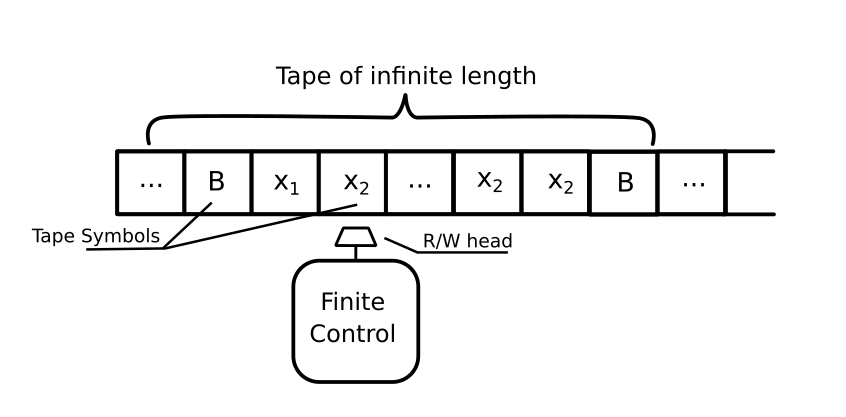
\includegraphics[scale=0.5]{TurigMachine.png}    
\caption{Turing Machine Concept - https://iq.opengenus.org/content/images/2019/07/TurigMachine.png}
\end{center}
\end{figure}

Head moves from one square to the next square and executes sets of instructions in sequence. We can think of heads as PC(Program Counter) in MIPS assembly, or IP(Instruction Pointer) in x86 architectures. In a Turing machine, the head reads and writes symbols on the tape and moves along the tape according to a set of rules that determine the next state of the machine. The position of the head on the tape represents the current state of the machine, and the tape contains both the data being processed and the instructions for the machine. 

\subsection{Stored Program}
In the mid-1940s, John von Neumann and his friends introduced a concept named "Stored Program". This was a way to design computers that could execute instructions stored in the memory. The basic idea was to store both data and instructions in the same memory, and to use a program counter to keep track of the address of the next instruction to be executed. 

\subsection{Summary}
Since this is a computer architecture class, I thought that those two concepts were worth mentioning before we start designing and implementing the program. In order to implement \texttt{mipsim}, I tried to implement it in a way that as much mimics the workflow of computers. For specific considerations on implementations, we are going to discuss them in the next section.

\pagebreak
\section {Design \& Implementation}
\subsection{Background}
Of course, there might be more core design principles when it comes to designing a program, there were two major considerations for this program:
\begin{itemize}
    \item \textbf{Stability}: The program shall be stable, meaning that the program must have "graceful" error handling rather than \texttt{SEGSEGV}.
    \item \textbf{Extensibility}: The program shall be easy to add some extra features in the future, such as new instructions and new registers.
\end{itemize}

In order for making those two principles alive, the program was designed in two major components:
\begin{itemize}
    \item \textbf{Assembler}: A component that reads file from user and makes it into a instruction that will be performed by the simulator in the future.
    \item \textbf{Simulator}: A component that actually executes instructions that were generated by assembler accordingly.
\end{itemize}
There were more minor components that were involved in this program to run smooth. Besides those requirements from Professor Nam, I have added some more requirements that will make this program perform better:

\begin{itemize}
    \item \textbf{Error Detection}: When the input file that the program was processing had an error, the program is required to tell user at which line there seems to be an error. For now, this only detects syntax errors instead of logical errors like infinite loops.
    \item \textbf{Command Line Interface}: For ease of use for users, a simple command line interface was supported. Such includes specifying an input file, specifying an output file. 
\end{itemize}

\subsection{Design Components}
\subsubsection{Assembler}
As the requirements of \texttt{HW1.pdf} suggests, the user will input assembly-like instructions inside a file. In order for the program to execute instructions from string, the program first needs to parse those strings into instructions. The assemble was designed to perform this task. In short, the assembler will read the file provided by the user line by line and store them as an array of instructions. Those instructions will be stored inside the memory and will be executed later by simulator.

One might ask, "why not execute string instructions line by line instead of storing them inside a memory?". Well, there are three main reasons for current design: reading all file and storing them as instructions:

\begin{itemize}
    \item \textbf{Mimic Stored Program}: Since we are studying computer architecture class, I just wanted to make this program mimic \textit{stored program} concept introduced by \textit{John von Neumann}. 
    \item \textbf{Speed and Optimization}: Since the program will read input file, parse string and execute instruction accordingly, the speed of executing a single instruction compared to stored instructions will be far slower due to the fact that there will be more IO operations involved. Not only does it require more IO operations, but there will be redundancy issues. For example, when a specific line of input is executed multiple times due to operations like \texttt{jmp} or \texttt{beq}, the program will perform the same operation to parse string into instructions multiple times. Therefore, for speed and optimization, stored instructions method was preferred.
    \item \textbf{Error Detection}: Since one of the requirements that this program has to offer were error detection, with assembler it will be easier to implement syntax error detection rather than line by line execution. Since the assembler will read all the lines before executing and check whether there is an error or not, the program will be more stable since it will have little chance of executing some unverified code that might have potential of bugs and errors.
\end{itemize}

\subsubsection{Simulator}
Implementing a simulator is rather a simple process compared to assembler. The simulator will take current context of simulation and execute the user's instruction that was requested. To mimic real computer operations, the simulator works with a simple variable named \texttt{pc}. Also, the simulator was designed with as much error handling as possible. For details on limitations on simulator, please check later section for more information.

\subsection{Implementation}
\subsubsection{Type Definitions}
Before starting to talk about details on implementations, we will now talk about type definitions first. There are some data types that were defined in the program for implementing the simulator. Those definitions can be found under \texttt{common.h}.

The first is the user's instructions and parameters. Those are tightly coupled together for future use.
\\
\begin{center}
\begin{code}
\begin{minted}[frame=single,framesep=10pt]{c}
struct param_t {
    uint32_t value;
    uint8_t type; // Distinguish registers from constants. 
};

struct user_instruction_t {
    uint8_t instruction;
    struct param_t param[3];
    uint8_t param_count;
};
\end{minted}
\captionof{listing}{Definition of \texttt{struct user_instruction_t} and \texttt{struct param_t}}
\end{code}
\end{center}

\texttt{struct user_instruction_t} are stored inside an array to mimic \textit{stored program} concept. This array will be used later inside the simulator.

The second is the context. Since the simulator needs to keep track of current contexts, such as PC and register states, the data type was introduced.
\\
\begin{center}
\begin{code}
\begin{minted}[frame=single,framesep=10pt]{c}
struct context_t {
    char input_file[MAX_STRING];
    char output_file[MAX_STRING];
    FILE *in_fp;
    FILE *out_fp;
    uint32_t pc;
    uint32_t registers[REGISTER_COUNT];
    uint16_t used_map;
    uint32_t last_instruction;
    struct user_instruction_t user_instructions[MAX_INSTRUCTION_COUNT];
};
\end{minted}
\captionof{listing}{Definition of \texttt{struct context_t}}
\end{code}
\end{center}

\texttt{struct context_t} store major information such as input file, output file, register status with their values and user's instructions. In order to keep track of used registers, this program uses \texttt{uint16_t} to store whether a specific register was used or not. LSB represents 0th register's status, if marked 1 this means that the register was being used. Since there are only 10 registers available, \texttt{uint16_t} was considered enough to represent all registers. 

The last type definition is the instruction. In order to save the syntax and function pointers of a specific instruction, this data type was introduced.
\\
\begin{center}
\begin{code}
\begin{minted}[frame=single,framesep=10pt]{c}
struct instruction_t {
    enum TokenType syntax[MAX_TOKEN_COUNT];
    uint8_t token_count;
    int (*function)(struct context_t *, struct user_instruction_t);
    char name[MAX_NAME_LEN];
};
\end{minted}
\captionof{listing}{Definition of \texttt{struct instruction_t}}
\end{code}
\end{center}

At the start of the program, all available instructions are turned into an array of \texttt{struct instruction_t}. Then with this instructions, the program checks predefined syntax. Also, for implementing "polymorphism", function pointer was used to call the function that actually executes the instruction. 

With those newly defined data types, the program performs syntax checking, assembling and simulating operations. 

\pagebreak

\subsubsection{Overview}
This program works in following sequence with give input file:
\\
\begin{figure}[h]
\begin{center}
\begin{tikzpicture}[node distance=2cm]

\node (input) [io] {Input File};
\node (syntax) [process, right of=input, xshift=2cm] {Syntax Checker};
\node (assemble) [process, right of=syntax, xshift=2cm] {Assembler};
\node (simulate) [process, right of=assemble, xshift=2cm] {Simulator};

\draw [arrow] (input) -- (syntax);
\draw [arrow] (syntax) -- (assemble);
\draw [arrow] (assemble) -- (simulate);

\end{tikzpicture}
\caption{Syntax Checker Flowchart}
\end{center}
\end{figure}
\\
From now on, we are going to talk about each sequences one by one. Actually, syntax checking and assembling is taken place at the same time. However, for ease of description, we are going to talk about each topics one by one.

\subsubsection{Syntax Checker}
Syntax checker verifies syntax of user's input file. The program will read line by line from the user's input file and store it as a \texttt{string}. Once the string was stored, it will check for syntax and verify if the input was valid or not. Again, keep in mind that syntax checker is actually implemented with the assembler in the code. For easy explanation, we are going to separate them in this document. The syntax checker works in following sequence as flowchart shows below:

\begin{figure}[h]
\begin{center}
\begin{tikzpicture}[node distance=2cm]

\node (input) [io] {Input};
\node (verify) [process, right of=input, xshift=2cm] {Verify Instruction};
\node (parse) [process, right of=verify, xshift=2cm] {Parse Param};
\node (syntax) [process, right of=parse, xshift=2cm] {Verify Syntax};

\draw [arrow] (input) -- (verify);
\draw [arrow] (verify) -- (parse);
\draw [arrow] (parse) -- (syntax);

\end{tikzpicture}
\caption{Syntax Checker Flowchart}
\end{center}
\end{figure}

\begin{enumerate}
    \item Syntax checker will verify the instruction. For example, if the user's input was \texttt{LW r0 0x5}, this step will verify that the instruction was given as \texttt{lw}. 
    \item Syntax checker will parse parameters. This will distinguish a constant from register. For example, if \texttt{r0} was given, it will parse it as register. On the other hand, \texttt{0x5} will be parsed as a constant. Also, in this step, each parameters will be stored as \texttt{struct param_t} type to indicate the type of parameter.
    \item Syntax checker will verify syntax. In this step, the program will check if the types of each parameters that were parsed from previous step was in a valid syntax. Details on this step will be discussed right below.
\end{enumerate}

Now, it is time to discuss about how syntax checker verifies if a syntax is valid or not. When the program loads, the program will automatically generate a predefined syntax of each instructions. Then it will compare each given parameter's types with the predefined syntax. To implement this, as we all know, there are three types of arguments for each different instructions:
\begin{itemize}
    \item \textbf{Register}: The register information.
    \item \textbf{Constant}: The constant value which are represented as hexadecimal.
    \item \textbf{Both}: Either register or constant works.
\end{itemize}

As Professor Nam requested, we can represent syntax of each instructions like following table:
\\
\\
\begin{figure}[h]
\begin{center}
\begin{tabular}{|l|l|l|}
    \hline
        \textbf{Name} & \textbf{Syntax} & \textbf{Token Count} \\
    \hline
        add & Register, Register, Register & 3 \\
        sub & Register, Register, Register & 3 \\
        mul & Register, Register, Register & 3 \\
        div & Register, Register, Register & 3 \\
        mov & Register, Both & 2 \\
        lw & Register, Constant & 2 \\
        sw & Register & 1 \\
        rst & & 0 \\
        jmp & Constant & 1 \\
        beq & Both, Both, Constant & 3 \\
        bne & Both, Both, Constant & 3 \\
        slt & Register, Both, Both & 3 \\
    \hline
\end{tabular}
\caption{Syntax Table of Instructions}
\end{center}
\end{figure}
\\
For ease of implementation, two instructions were implemented in a slightly modified way:

\begin{itemize}
    \item \texttt{rst}: Originally required format of \texttt{rst \$register STDOUT}. However, in order to implement the program a bit easier, this program omits \texttt{STDOUT} since there is just only one option. 
    \item \texttt{slt}: Originally the first argument was fixed as \texttt{\$r0}, however this program supports other registers as well. 
\end{itemize}

As we construct this table, it will be easier for us to implement the syntax checking feature. With this table, by comparing each instruction's type with the predefined syntax, we can achieve syntax checking. 

Let's check an example input below to see how this works.
\\
\begin{center}
\begin{code}
\begin{minted}[frame=single,framesep=10pt]{bash}
LW r0 0x5 # Load 0x5 to register 0
\end{minted}
\captionof{listing}{Example Input}
\end{code}
\end{center}

Before the program checks the syntax, it will drop everything after \texttt{\#} which are comments. In the first step, syntax checker will identify \texttt{LW} as instruction \texttt{lw}. Once it identifies the user's instruction, it will then parse each passed arguments. Since the code had \texttt{r0} and \texttt{0x5}, each will be parsed as \texttt{Register} and a \texttt{Constant}. Then, it will check syntax. Since we have a predefined syntax like below:
\\
\begin{center}
\begin{code}
\begin{minted}[frame=single,framesep=10pt]{c}
{ .syntax = {Register, Constant}, ... .name = "lw"},
\end{minted}
\captionof{listing}{Syntax Definition of \texttt{LW}}
\end{code}
\end{center}

The full code can be found under \texttt{generate_instructions} of \texttt{main.c}. Since the user's given syntax was in the correct sequence, \texttt{Register, Context} it will pass syntax check. Once the syntax was valid, the program will then move onto the next step: assembling.

\subsubsection{Assembler}
As mentioned earlier, while the syntax checker verifies for the syntax, it also generates instruction at the same time. The generated instruction will be stored as a \texttt{struct user_instruction_t} type for future use. For example, if we had a instruction like Code Snippet 4, the program will store instruction as following figure:

\begin{figure}[h]
  \centering
  \includesvg[inkscapelatex=false, width = 200pt]{ca-1.svg}
  \caption{Example of Storing Instruction}
\end{figure}

The figure is for your understanding. Some details were omitted for better explanation. Also, instruction 5 means that this was an \texttt{lw} instruction. The table of each instructions are as it follows:

\begin{figure}[h]
\centering
\begin{tabular}{ |c|c| }
  \hline
  Entry & Enum Value \\
  \hline
  Add & 0 \\
  Sub & 1 \\
  Mul & 2 \\
  Div & 3 \\
  Mov & 4 \\
  Lw & 5 \\
  Sw & 6 \\
  Rst & 7 \\
  Jmp & 8 \\
  Beq & 9 \\
  Bne & 10 \\
  Slt & 11 \\
  \hline
\end{tabular}
  \caption{Instruction ID Table}
\end{figure}

Then each instructions will be stored in memory as an array for simulation in the future. Once the assembler finishes converting a user input text into a \texttt{struct user_instruction_t} type data, it is now ready to be executed.

\subsubsection{Simulator}
Since syntax checking and assembling were finished, it is now time to start simulating each instructions. In each execution of instructions, there are 4 requirements that shall be satisfied:
\begin{enumerate}
    \item \textbf{Manage PC}: Since the simulator needs to direct the next instruction's address, in our case which is index, the simulator needs to manage PC before executing the instruction.
    \item \textbf{Execute}: The simulator must execute user's given instruction. Each instruction will be actually executed by functions accessed by function pointers.
    \item \textbf{Output}: One of the requirements of this program was to show internal state of registers when being used. Also if we had some \texttt{STDOUT} related jobs, the program must print it out in the screen as well.
    \item \textbf{Dump}: The program stores each execution results into a file. Therefore, it shall dump data into the file when executing a single instruction.
\end{enumerate}

Simulator simulates the user instruction with following simple algorithm.

\begin{algorithm}
\caption{Simulator Algorithm}\label{alg:cap}
\begin{algorithmic}
    \Procedure{execute}{$ctx$}
    \While{$ctx.pc \neq ctx.lastInstruction$}
        \State $ctx.pc$ \gets $ctx.pc + 1$ \Comment{Increment PC}
        \State Execute instruction
        \If{Error Found}
            \State Quit
        \EndIf
        \If $ctx.pc > ctx.lastInstruction$ \Comment{When PC was jumped too far}
            \State Quit
        \EndIf
        \State Print register stats and dump info file
    \EndWhile
\end{algorithmic}
\end{algorithm}

Each user instructions are executed by function pointers that are loaded in the memory when the program starts. For example with Code Snippet 4, which performs \texttt{lw} instruction, the simulator will first set PC to the next instruction. After that, it will call callback function for actually executing the instruction. The \texttt{lw} instruction uses \texttt{sim_lw} function to execute instruction. Therefore, following code will be executed using function pointer:
\\
\begin{center}
\begin{code}
\begin{minted}[frame=single,framesep=10pt]{c}
int sim_lw(struct context_t *ctx, struct user_instruction_t instruction) {
    uint32_t constant = instruction.param[1].value;
    uint32_t *dst = &ctx->registers[instruction.param[0].value];
    *dst =  constant;

    mark_registers(ctx, instruction);
    return 0;
}
\end{minted}
\captionof{listing}{Callback Function for \textt{LW}}
\end{code}
\end{center}
\\
After simulator executes \texttt{sim_lw}, it will check for errors and verify if the execution context is correct. For example some operations like \texttt{jmp}, \texttt{bne} and \texttt{beq} does not check if the address that it is jumping to is valid or not. Therefore, in verification step, the simulator will check if the simulation is being performed well or not. Also the simulator will print data out to the user screen and store output to file as well. The simulator will continue execution until it hits the last instruction. Once it hits the end of the instructions, it will quit execution gracefully. 

With simple algorithm, simulator can execute user instructions until it meets the last instruction in designated file. 

\subsubsection{Summary}
In short, \texttt{mipsim} has three major parts: syntax checker, assembler and simulator. Syntax checker checks and verifies user's input with predefined syntax. At the same time, assembler converts each strings of user's lines into \texttt{struct user_instruction_t} which will be used later. Once syntax checker and assembler finishes their job, the simulator starts executing stored instructions one by one. If you would like to see the actions in code, please check \texttt{simulator.c}, \texttt{syntax.c} and \texttt{io.c} for more information. All functions and definitions have rich documentation, therefore it will be easy to understand what is going on with the code.
\pagebreak

\section{User Guide & Environments}
\subsection{Environment}
The environment that this program was checked running is as it follows:
\begin{itemize}
    \item \textbf{OS}: Ubuntu 22.04.01 LTS
    \item \textbf{CPU}: Intel(R) Core(TM) i9-7940X CPU @ 3.10GHz
    \item \textbf{RAM}: 64GB
    \item \textbf{Compiler}: GCC 11.3.0, Make 4.3
    \item \textbf{C}: C99
\end{itemize}

Please be aware that with some environments, the program might not be able to execute. Also, with the code was zipped with version \texttt{Zip 3.0}. 

\subsection{User Guide}
\subsubsection{Unzipping}
Once you have downloaded the attached \texttt{.zip} file, you first need to unzip the file using following command.
\\
\begin{center}
\begin{code}
\begin{minted}[frame=single,framesep=10pt]{bash}
$ unzip FILE_NAME.zip
\end{minted}
\captionof{listing}{Unzip Command Example}
\end{code}
\end{center}
\\
Please change the \texttt{FILE_NAME.zip} to the file that I have attached accordingly.

\subsubsection{Building}
Once you have unzipped the attatched file, there will be a directory named \texttt{mipsim}. Navigate to the directory \texttt{mipsim} by using \texttt{cd}. \texttt{mipsim} supports \texttt{make} with following recipes:
\begin{itemize}
    \item \texttt{debug}: For building debug version executable program with \texttt{--DDEBUG} option.
    \item \texttt{all}: For building executable program.
    \item \texttt{clean}: For cleaning up all \texttt{.o} files and generated executable program.
\end{itemize}

For example, if you were to build yourself a version for end-user case, use following command:
\\
\begin{center}
\begin{code}
\begin{minted}[frame=single,framesep=10pt]{bash}
$ make
gcc -O2 -Wall -std=gnu99 -o context.o -c context.c
gcc -O2 -Wall -std=gnu99 -o io.o -c io.c
gcc -O2 -Wall -std=gnu99 -o simulator.o -c simulator.c
gcc -O2 -Wall -std=gnu99 -o syntax.o -c syntax.c
gcc -O2 -Wall -std=gnu99 -o main.o -c main.c
gcc -o mipsim context.o io.o simulator.o syntax.o main.o
\end{minted}
\captionof{listing}{Example Build Output}
\end{code}
\end{center}
\\
This will generate object files ending with \texttt{.o} as well as an executable file named \texttt{mipsim}. To clean up your workspace, use \texttt{clean} recipe for removing all generated files.

\subsubsection{User Guide}
\texttt{mipsim} offers simple command line interfaces. You can use following command to get a glimpse of each options:
\\
\begin{center}
\begin{code}
\begin{minted}[frame=single,framesep=10pt]{bash}
$ ./mipsim  --help
...
                    A Simple MIPS Calculator
                            32190984 Isu Kim
Usage: mipsim [options]
Options
  -h, --help           Print this help message and exit
  -i, --input          Specify an input file to execute
  -o, --output         Specify an output file to dump log into
\end{minted}
\captionof{listing}{Example Help Output}
\end{code}
\end{center}

The options are:
\begin{itemize}
    \item \texttt{help}: For printing out the help message.
    \item \texttt{input}: For specifying an input file. This is required parameter.
    \item \texttt{output}: For specifying the output file. This will write execution results to the specified file. If not specified, the file will default to \texttt{out.txt}.
\end{itemize}

For example, an example execution command will be:
\\
\begin{center}
\begin{code}
\begin{minted}[frame=single,framesep=10pt]{bash}
$ ./mipsim  -i input.txt -o output.txt
...
                    A Simple MIPS Calculator
                            32190984 Isu Kim
[INFO] Input File: input.txt
[INFO] Output File: output.txt
\end{minted}
\captionof{listing}{Example Command Line Interface Output}
\end{code}
\end{center}

This will execute an file named \texttt{input.txt} and store results to \texttt{output.txt}. 

\warningbox{As defined in \texttt{common.h}, the maximum length of input is 1024 characters. File names that are longer than 1024 characters will have unexpected behaviors.}

\pagebreak
\subsubsection{Available Instructions}
\\
\begin{figure}[h]
\begin{center}
\begin{tabular}{|l|l|l|l|l|}
    \hline
        \textbf{Name} & \textbf{Syntax} & \textbf{Token Count} & \textbf{Available} & \textbf{Callback Function}\\
    \hline
        add & Register, Register, Register & 3 & O & \texttt{sim_add}\\
        sub & Register, Register, Register & 3 & O & \texttt{sim_sub}\\
        mul & Register, Register, Register & 3 & O & \texttt{sim_mul}\\
        div & Register, Register, Register & 3 & O & \texttt{sim_div}\\
        mov & Register, Both & 2 & O & \texttt{sim_mov}\\
        lw & Register, Constant & 2 & O & \texttt{sim_lw}\\
        sw & Register & 1 & O & \texttt{sim_sw}\\
        rst & & 0 & O & \texttt{sim_rst}\\
        jmp & Constant & 1 & O & \texttt{sim_jmp}\\
        beq & Both, Both, Constant & 3 & O & \texttt{sim_beq}\\
        bne & Both, Both, Constant & 3 & O & \texttt{sim_bne}\\
        slt & Register, Both, Both & 3 & O & \texttt{sim_slt}\\
    \hline
\end{tabular}
\caption{Table of Available Instructions}
\end{center}
\end{figure}
\\
Each implementation of callback functions can be found under \texttt{simulator.c}. Since mentioning all the functions one by one seems redundant, we are not going to discuss about each functions. Each functions have quite rich documentation, therefore it will be better to check the source code.  

\subsubsection{Demonstrations}
In order to verify if \texttt{mipsim} works properly or not, the list below is the codes that were tested working on \texttt{mipsim}. Also codes are included in the attachments, so you can try them yourself.

\begin{figure}[h]
\begin{center}
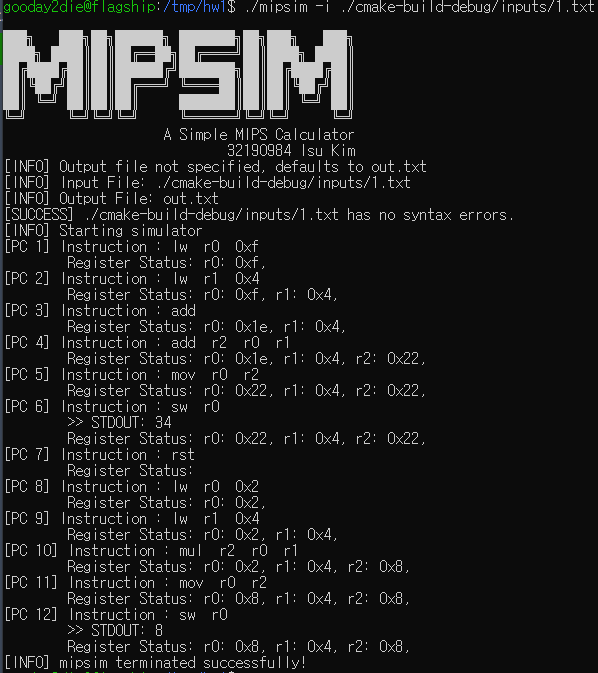
\includegraphics[scale=0.5]{mipsim.png}    
\caption{Example Execution Screenshot}
\end{center}
\end{figure}

The screenshot is an example executing \texttt{mipsim}. Since this picture was difficult for me to recognize the results, I will be copying the execution results into this document instead of attaching some screenshots.

All the codes the examples mentioned above can be found under the directory \texttt{inputs}. You can test the following codes out yourself to check \texttt{mipsim}:
\begin{itemize}
    \item \texttt{input/1.txt}: Basic execution from page 5 of \texttt{HW1.pdf}.
    \item \texttt{input/2.txt}: Basic execution from page 6 of \texttt{HW1.pdf}.
    \item \texttt{input/3.txt}: Basic execution from far left side code page 7 of \texttt{HW1.pdf}.
    \item \texttt{input/4.txt}: Basic execution from far right side code page 7 of \texttt{HW1.pdf}.
    \item \texttt{input/e1.txt}: Error execution with 3 syntax errors.
    \item \texttt{input/e2.txt}: Error execution with wrong addressing.
    \item \texttt{input/l1.txt}: Loop execution for 10 times. Prints out 4, 8, 12, ... 40.
\end{itemize}
\\
\\
\begin{center}
\begin{code}
\begin{minted}[frame=single,framesep=10pt]{bash}
LW r0 0xF # The second operand is a number
LW r1 0x4
ADD r2 r0 r1
MOV r0 r2
SW r0 STDOUT # STDOUT is a signal to print out $r0
RST # Reset all registers
LW r0 0x2
LW r1 0x4
MUL r2 r0 r1
MOV r0 r2
SW r0 STDOUT
\end{minted}
\captionof{listing}{Example Code \texttt{input/1.txt}}
\end{code}
\end{center}
\\
Also for demonstration of dump file, we are going to store result data into \texttt{./outputs/1.txt}. Therefore, an example execution will be as it follows:
\\
\begin{center}
\begin{code}
\begin{minted}[frame=single,framesep=10pt]{bash}
$ ./mipsim  -i inputs/1.txt -o output/1.txt
...
[INFO] Input File: inputs/1.txt
[INFO] Output File: output/1.txt
[SUCCESS] inputs/1.txt has no syntax errors.
[INFO] Starting simulator
[PC 1] Instruction : lw  r0  0xf
        Register Status: r0: 0xf,
[PC 2] Instruction : lw  r1  0x4
        Register Status: r0: 0xf, r1: 0x4,
[PC 3] Instruction : add  r2  r0  r1
        Register Status: r0: 0xf, r1: 0x4, r2: 0x13,
[PC 4] Instruction : mov  r0  r2
        Register Status: r0: 0x13, r1: 0x4, r2: 0x13,
[PC 5] Instruction : sw  r0
        >> STDOUT: 19
        Register Status: r0: 0x13, r1: 0x4, r2: 0x13,
[PC 6] Instruction : rst
        Register Status:
[PC 7] Instruction : lw  r0  0x2
        Register Status: r0: 0x2,
[PC 8] Instruction : lw  r1  0x4
        Register Status: r0: 0x2, r1: 0x4,
[PC 9] Instruction : mul  r2  r0  r1
        Register Status: r0: 0x2, r1: 0x4, r2: 0x8,
[PC 10] Instruction : mov  r0  r2
        Register Status: r0: 0x8, r1: 0x4, r2: 0x8,
[PC 11] Instruction : sw  r0
        >> STDOUT: 8
        Register Status: r0: 0x8, r1: 0x4, r2: 0x8,
[INFO] mipsim terminated successfully!
\end{minted}
\captionof{listing}{Example Execution Output for \texttt{input/1.txt}}
\end{code}
\end{center}
\\
Since the code did not have any errors, \texttt{mipsim} executes the code without any issues. In \texttt{output/1.txt}, following dump is stored:
\\
\begin{center}
\begin{code}
\begin{minted}[frame=single,framesep=10pt]{bash}
$ cat output/1.txt
Instruction : lw  r0  0xf
        Registers: r0: 0xf,
Instruction : lw  r1  0x4
        Registers: r0: 0xf, r1: 0x4,
Instruction : add  r2  r0  r1
        Registers: r0: 0xf, r1: 0x4, r2: 0x13,
Instruction : mov  r0  r2
        Registers: r0: 0x13, r1: 0x4, r2: 0x13,
Instruction : sw  r0
        Registers: r0: 0x13, r1: 0x4, r2: 0x13,
Instruction : rst
        Registers:
Instruction : lw  r0  0x2
        Registers: r0: 0x2,
Instruction : lw  r1  0x4
        Registers: r0: 0x2, r1: 0x4,
Instruction : mul  r2  r0  r1
        Registers: r0: 0x2, r1: 0x4, r2: 0x8,
Instruction : mov  r0  r2
        Registers: r0: 0x8, r1: 0x4, r2: 0x8,
Instruction : sw  r0
        Registers: r0: 0x8, r1: 0x4, r2: 0x8,
\end{minted}
\captionof{listing}{Example Execution Dump for \texttt{input/1.txt}}
\end{code}
\end{center}

Following output is for demonstrating the \texttt{input/2.txt}'s execution. 
\\
\begin{center}
\begin{code}
\begin{minted}[frame=single,framesep=10pt]{bash}
$ ./mipsim  -i inputs/2.txt -o output/2.txt
...
[INFO] Input File: inputs/2.txt
[INFO] Output File: output/2.txt
[SUCCESS] inputs/2.txt has no syntax errors.
[INFO] Starting simulator
[PC 1] Instruction : lw  r0  0x5
        Register Status: r0: 0x5,
[PC 2] Instruction : lw  r1  0xf
        Register Status: r0: 0x5, r1: 0xf,
[PC 3] Instruction : add  r2  r0  r1
        Register Status: r0: 0x5, r1: 0xf, r2: 0x14,
[PC 4] Instruction : jmp  0x9
        Register Status: r0: 0x5, r1: 0xf, r2: 0x14,
[PC 9] Instruction : add  r3  r1  r2
        Register Status: r0: 0x5, r1: 0xf, r2: 0x14, r3: 0x23,
[PC 10] Instruction : mov  r0  r3
        Register Status: r0: 0x23, r1: 0xf, r2: 0x14, r3: 0x23,
[PC 11] Instruction : sw  r0
        >> STDOUT: 35
        Register Status: r0: 0x23, r1: 0xf, r2: 0x14, r3: 0x23,
[INFO] mipsim terminated successfully!
\end{minted}
\captionof{listing}{Example Execution Output for \texttt{input/2.txt}}
\end{code}
\end{center}
\\
Following output is for demonstrating the \texttt{input/3.txt}'s execution. 
\\
\begin{center}
\begin{code}
\begin{minted}[frame=single,framesep=10pt]{bash}
$ ./mipsim  -i inputs/3.txt -o output/3.txt
...
[INFO] Input File: inputs/3.txt
[INFO] Output File: output/3.txt
[SUCCESS] inputs/3.txt has no syntax errors.
[INFO] Starting simulator
[PC 1] Instruction : lw  r0  0x5
        Register Status: r0: 0x5,
[PC 2] Instruction : lw  r1  0xa
        Register Status: r0: 0x5, r1: 0xa,
[PC 3] Instruction : bne  r0  r1  0x6
        Register Status: r0: 0x5, r1: 0xa,
[PC 6] Instruction : mov  r0  0x1
        Register Status: r0: 0xa, r1: 0xa,
[PC 7] Instruction : sw  r0
        >> STDOUT: 10
        Register Status: r0: 0xa, r1: 0xa,
[INFO] mipsim terminated successfully!
\end{minted}
\captionof{listing}{Example Execution Output for \texttt{input/3.txt}}
\end{code}
\end{center}
\\
Following output is for demonstrating the \texttt{input/4.txt}'s execution. 
\\
\begin{center}
\begin{code}
\begin{minted}[frame=single,framesep=10pt]{bash}
$ ./mipsim  -i inputs/4.txt -o output/4.txt
...
[INFO] Input File: inputs/4.txt
[INFO] Output File: output/4.txt
[SUCCESS] inputs/4.txt has no syntax errors.
[INFO] Starting simulator
[PC 1] Instruction : lw  r0  0x5
        Register Status: r0: 0x5,
[PC 2] Instruction : lw  r1  0xa
        Register Status: r0: 0x5, r1: 0xa,
[PC 3] Instruction : slt  r2  r0  r1
        Register Status: r0: 0x5, r1: 0xa, r2: 0x1,
[PC 4] Instruction : bne  r0  0x0  0x7
        Register Status: r0: 0x5, r1: 0xa, r2: 0x1,
[PC 7] Instruction : mov  r0  0x1
        Register Status: r0: 0xa, r1: 0xa, r2: 0x1,
[PC 8] Instruction : sw  r0
        >> STDOUT: 10
        Register Status: r0: 0xa, r1: 0xa, r2: 0x1,
[INFO] mipsim terminated successfully!
\end{minted}
\captionof{listing}{Example Execution Output for \texttt{input/4.txt}}
\end{code}
\end{center}
\\

As you can see, the executions were performed without any issues. Now, let's test some cases with errors. Let's use a code that has three errors.
\\
\begin{center}
\begin{code}
\begin{minted}[frame=single,framesep=10pt]{bash}
LW r0 r2 # Second needs to be constant
LW r1 0x4
ADD r2 r0 0x3 # Third needs to be register
MOV r0 r2
SW r0 STDOUT
RST
LW r0 0x2
LW r1 0x4
MUL 0x4 r0 r1 # First needs to be register
MOV r0 r2
SW r0 STDOUT
\end{minted}
\captionof{listing}{Example Erroneous Code \texttt{input/e1.txt}}
\end{code}
\end{center}
\\
The code has three syntax errors. When we execute the code with \texttt{mipsim}, the result is as it follows:
\\
\begin{center}
\begin{code}
\begin{minted}[frame=single,framesep=10pt]{bash}
$ ./mipsim -i ./inputs/e1.txt
...
[INFO] Output file not specified, defaults to out.txt
[INFO] Input File: ./inputs/e1.txt
[INFO] Output File: out.txt
 - Syntax Error @ ln1
        invalid argument type: r2
        expected constant but got register
 - Syntax Error @ ln3
        invalid argument type: 0x3
        expected register but got constant
 - Syntax Error @ ln9
        invalid argument type: 0x4
        expected register but got constant
[ERROR] Found syntax error, exiting mipsim.
\end{minted}
\captionof{listing}{Example Erroneous Code Execution - \texttt{input/e1.txt}}
\end{code}
\end{center}
\\
\texttt{mipsim} catches three errors with reason. Since \texttt{mipsim} found errors in syntax checking and assembling phase, it will not start simulator. 
\par
Let's take a look into another case with a code that is correct in syntax however addresses unavailable address.
\\
\begin{center}
\begin{code}
\begin{minted}[frame=single,framesep=10pt]{bash}
LW r0 0x5
LW r1 0xF
ADD r2 r0 r1
JMP 0xF  # Line 15 does not exist
RST
LW r0 0x2
LW r1 0x4
MUL r2 r0 r0
ADD r3 r1 r2
MOV r0 r3
SW r0 STDOUT
\end{minted}
\captionof{listing}{Example Erroneous Code \texttt{input/e2.txt}}
\end{code}
\end{center}
\\
Since this was a code that was correct in syntax, syntax checker and assembler will consider this code valid. Therefore, the simulator will start operating. However, since the addressing was invalid, simulator will quit execution as soon as it hits the \texttt{jmp} instruction. An example output is like as it follows:
\\
\begin{center}
\begin{code}
\begin{minted}[frame=single,framesep=10pt]{bash}
$ ./mipsim -i ./cmake-build-debug/inputs/e2.txt
...
[INFO] Output file not specified, defaults to out.txt
[INFO] Input File: ./cmake-build-debug/inputs/e2.txt
[INFO] Output File: out.txt
[SUCCESS] ./cmake-build-debug/inputs/e2.txt has no syntax errors.
[INFO] Starting simulator
[PC 1] Instruction : lw  r0  0x5
        Register Status: r0: 0x5,
[PC 2] Instruction : lw  r1  0xf
        Register Status: r0: 0x5, r1: 0xf,
[PC 3] Instruction : add  r2  r0  r1
        Register Status: r0: 0x5, r1: 0xf, r2: 0x14,
[PC 4] Instruction : jmp  0xf
Invalid addressing while executing instruction @ ln15
\end{minted}
\captionof{listing}{Example Erroneous Code Execution - \texttt{input/e2.txt}}
\end{code}
\end{center}
\\
\texttt{mipsim} catches that the code instruction was using wrong address, therefore terminating program. Let's take a look at an example with loop using codes:
\\
\begin{center}
\begin{code}
\begin{minted}[frame=single,framesep=10pt]{bash}
LW r1 0x4  # Actually a constant 4
LW r2 0x1  # Actually a constant 1
LW r3 0x0  # i = 0
ADD r3 r3 r2  # i++
MUL r4 r1 r3  # a = i * 4
SW r4 STDOUT  # print a, shall print out 4, 8 ~ 40
SLT r0 r3 0xa  # i < 10
BEQ r0 0x1 0x4  # loop
\end{minted}
\captionof{listing}{Example Loop Code \texttt{input/l1.txt}}
\end{code}
\end{center}
\\
When we execute the program, \texttt{mipsim} prints out numbers 4, 8, 12, ~ 40 correctly like below:
\\
\begin{center}
\begin{code}
\begin{minted}[frame=single,framesep=10pt]{bash}
$ ./mipsim -i ./cmake-build-debug/inputs/l1.txt
...
[INFO] Output file not specified, defaults to out.txt
[INFO] Input File: ./cmake-build-debug/inputs/l1.txt
[INFO] Output File: out.txt
[SUCCESS] ./cmake-build-debug/inputs/l1.txt has no syntax errors.
[INFO] Starting simulator
[PC 1] Instruction : lw  r1  0x4
        Register Status: r1: 0x4,
[PC 2] Instruction : lw  r2  0x1
        Register Status: r1: 0x4, r2: 0x1,
[PC 3] Instruction : lw  r3  0x0
        Register Status: r1: 0x4, r2: 0x1, r3: 0x0,
[PC 4] Instruction : add  r3  r3  r2
        Register Status: r1: 0x4, r2: 0x1, r3: 0x1,
[PC 5] Instruction : mul  r4  r1  r3
        Register Status: r1: 0x4, r2: 0x1, r3: 0x1, r4: 0x4,
[PC 6] Instruction : sw  r4
        >> STDOUT: 4
...
        >> STDOUT: 8
...
         >> STDOUT: 40
Register Status: r0: 0x1, r1: 0x4, r2: 0x1, r3: 0xa, r4: 0x28,
[PC 7] Instruction : slt  r0  r3  0xa
        Register Status: r0: 0x0, r1: 0x4, r2: 0x1, r3: 0xa, r4: 0x28,
[PC 8] Instruction : beq  r0  0x1  0x4
        Register Status: r0: 0x0, r1: 0x4, r2: 0x1, r3: 0xa, r4: 0x28,
[INFO] mipsim terminated successfully!
\end{minted}
\captionof{listing}{Example Loop Code Execution - \texttt{input/l1.txt}}
\end{code}
\end{center}
\\
As the result shows, \texttt{mipsim} executes loop for 10 times and terminates successfully. 
\warningbox{\texttt{mipsim} does not have ability to detect infinite loops. Therefore, be extra cautious when writing loop codes.}

\subsection{Limitations and Extra Features}
\texttt{mipsim} was designed to implement as much as the original \texttt{HW1.pdf} requested. However, in some operations, the requirements were slightly changed due to limitations and for better experience. Please check following list for changes in instructions.
\begin{itemize}
    \item \texttt{sw}: The instruction will actually ignore token \texttt{STDOUT}. To reduce complexity in the code, the instruction was designed to print out the reigster value that was given as first argument. Therefore, the syntax checker will make some expressions without \texttt{STDOUT} as valid. 
    \item \texttt{sll}: The instruction originally was required to set \texttt{r0} as the result of comparing two registers or constants. However, for extra features, \texttt{mipsim} supports other registers to be used as well. Meaning that \texttt{sll r2 10 20} will store \texttt{r2} a value of 1. 
\end{itemize}
Besides instructions, there are limitations of the overall program:
\begin{itemize}
    \item \textbf{Maximum Input}: The maximum string length that \texttt{mipsim} can handle is 1024 bytes. Meaning that if you have a single line that exceeds 1024 characters, \texttt{mipsim} will drop the remaining part. 
    \item \textbf{Maximum Instructions}: In order to minimize memory overhead, \texttt{mipsim} offers maximum 1024 user instructions. Meaning that if you instructions more than 1024 instructions, \texttt{mipsim} will not be able to execute instructions correctly.
    \item \textbf{Register Size}: Each registers are stored as a \texttt{uint32_t} variable. Meaning that each registers are 32 bit. \texttt{mipsim} will not trap nor notify the user about register values overflowing.
    \item \textbf{Constant Size}: When you use a constant such as \texttt{0xFF}, the maximum value that \texttt{mipsim} can store is 32 bits. 
    \item \textbf{Character Set}: \texttt{mipsim} only supports \texttt{ASCII} characters, saving input fie using other character set such as \texttt{UNICODE} will have unexpected behaviors.
\end{itemize}

\pagebreak
\section{Conclusion}
Implementing \texttt{mipsim} was quite a fun project. Since we all learn the concept of "stored program" and "Turing machine", it was quite interesting to make a program that mimics the characteristics of those concepts. Also, when implementing \texttt{mipsim}, the following list represents the encountered difficulties:

\begin{itemize}
    \item \textbf{Parsing String}: C has some powerful library named \texttt{string.h} for dealing with strings. However, compared to other languages which supports easy use of string related functions, using strings in \texttt{C} is quite difficult. For example, using \texttt{strtok} compared to \texttt{.split()} method from Python is quite challenging. 
    \item \textbf{Designing}: Designing \texttt{mipsim} to become extensible was quite challenging process. There were lots of considerations when implementing \texttt{mipsim} since the program itself was quite simple. However, keeping design principles throughout the project was quite difficult process.
    \item \textbf{Environment}: Professor Nam told us that if he could not create an environment himself by this manual, he will not grade the project. In order for this project to be graded, I considered using from \texttt{Docker} to using \texttt{Vagrant}. However, since the code is quite simple and does not require external libraries, it was preferred to use basic \texttt{C} and \texttt{make} commands. 
\end{itemize}

While implementing this project, there were some features that I thought that might come in handy when adding more instructions:
\begin{itemize}
    \item \textbf{Memory}: Since current \texttt{lw} and \texttt{sw} does not store extra data in memory, it was considered to be a good idea to construct a virtual memory. 
    \item \textbf{Branches}: Since current code uses direct line count for \texttt{jmp}, \texttt{beq} and \texttt{bne}, it would have been better if we add a branch feature. Meaning that instead of using \texttt{jmp 0x10}, using \texttt{jmp label} will jump us to the corresponding line as well. 
\end{itemize}

Also, while designing and implementing \texttt{mipsim}, there were some things that I was able to recall and review:
\begin{itemize}
    \item \texttt{C}: Since the last time that I wrote a genuine \texttt{C} code was last semester, yes there were some codes like \texttt{eBPF} which doesn't count, it was nice to recall some techniques and important concepts in \texttt{C}. Such includes: function pointers and string parsing.
    \item \textbf{Designing}: Designing a program and defining requirements before implementing a program was a good practice in this project. Avoiding to code before designing the program saved lots of time.
\end{itemize}

I pretty much enjoyed implementing \texttt{mipsim} and would like to add those features mentioned up above in the future. 

\end{document}
